\chapter{\texorpdfstring{Workflow Modules and Systems}{Workflow Modules and Systems}}
\label{ch:18}
\lecturemeta{Lezione 18 \quad\textbullet\quad 2026-07-04 \quad\textbullet\quad Roberto Bruni}{Weske, \emph{Business Process Management}, Ch.6}

Nella lezione su \hyperref[ch:16b]{BPMN} abbiamo visto un caso sorprendente: due workflow \textbf{sound} presi singolarmente (Buyer 3 e Reseller 2) diventavano \textbf{non sound} una volta messi in comunicazione. Questa lezione formalizza \emph{perché} succede e \emph{come} analizzarlo: introduciamo i \textbf{workflow module} (un workflow net con un'interfaccia di comunicazione) e i \textbf{workflow system} (più moduli composti insieme), per poi mostrare che la soundness composta va verificata sul \textbf{sistema completo}, non sui pezzi.

\section{\texorpdfstring{Il problema: interazione fra processi}{Il problema: interazione fra processi}}

Un workflow net, per come l'abbiamo definito finora, è un mondo chiuso: nessun task dipende da eventi esterni. Ma nella realtà \textbf{non tutti i task sono automatici}: alcuni sono innescati da un \textbf{messaggio} in arrivo, altri \textbf{inviano} un messaggio per innescare un task altrove.

\begin{boxnote}{Interazione implicita}
Le attività di un processo possono: - \textbf{ricevere} un messaggio (simbolo \textbf{?}, es. \texttt{?rec\_accept}); - \textbf{inviare} un messaggio (simbolo \textbf{!}, es. \texttt{!accept}).

Finché il processo è visto da solo, questi simboli sono solo un'annotazione — un promemoria che quell'attività interagisce con l'esterno.
\end{boxnote}

\begin{figure}[!htb]
\centering
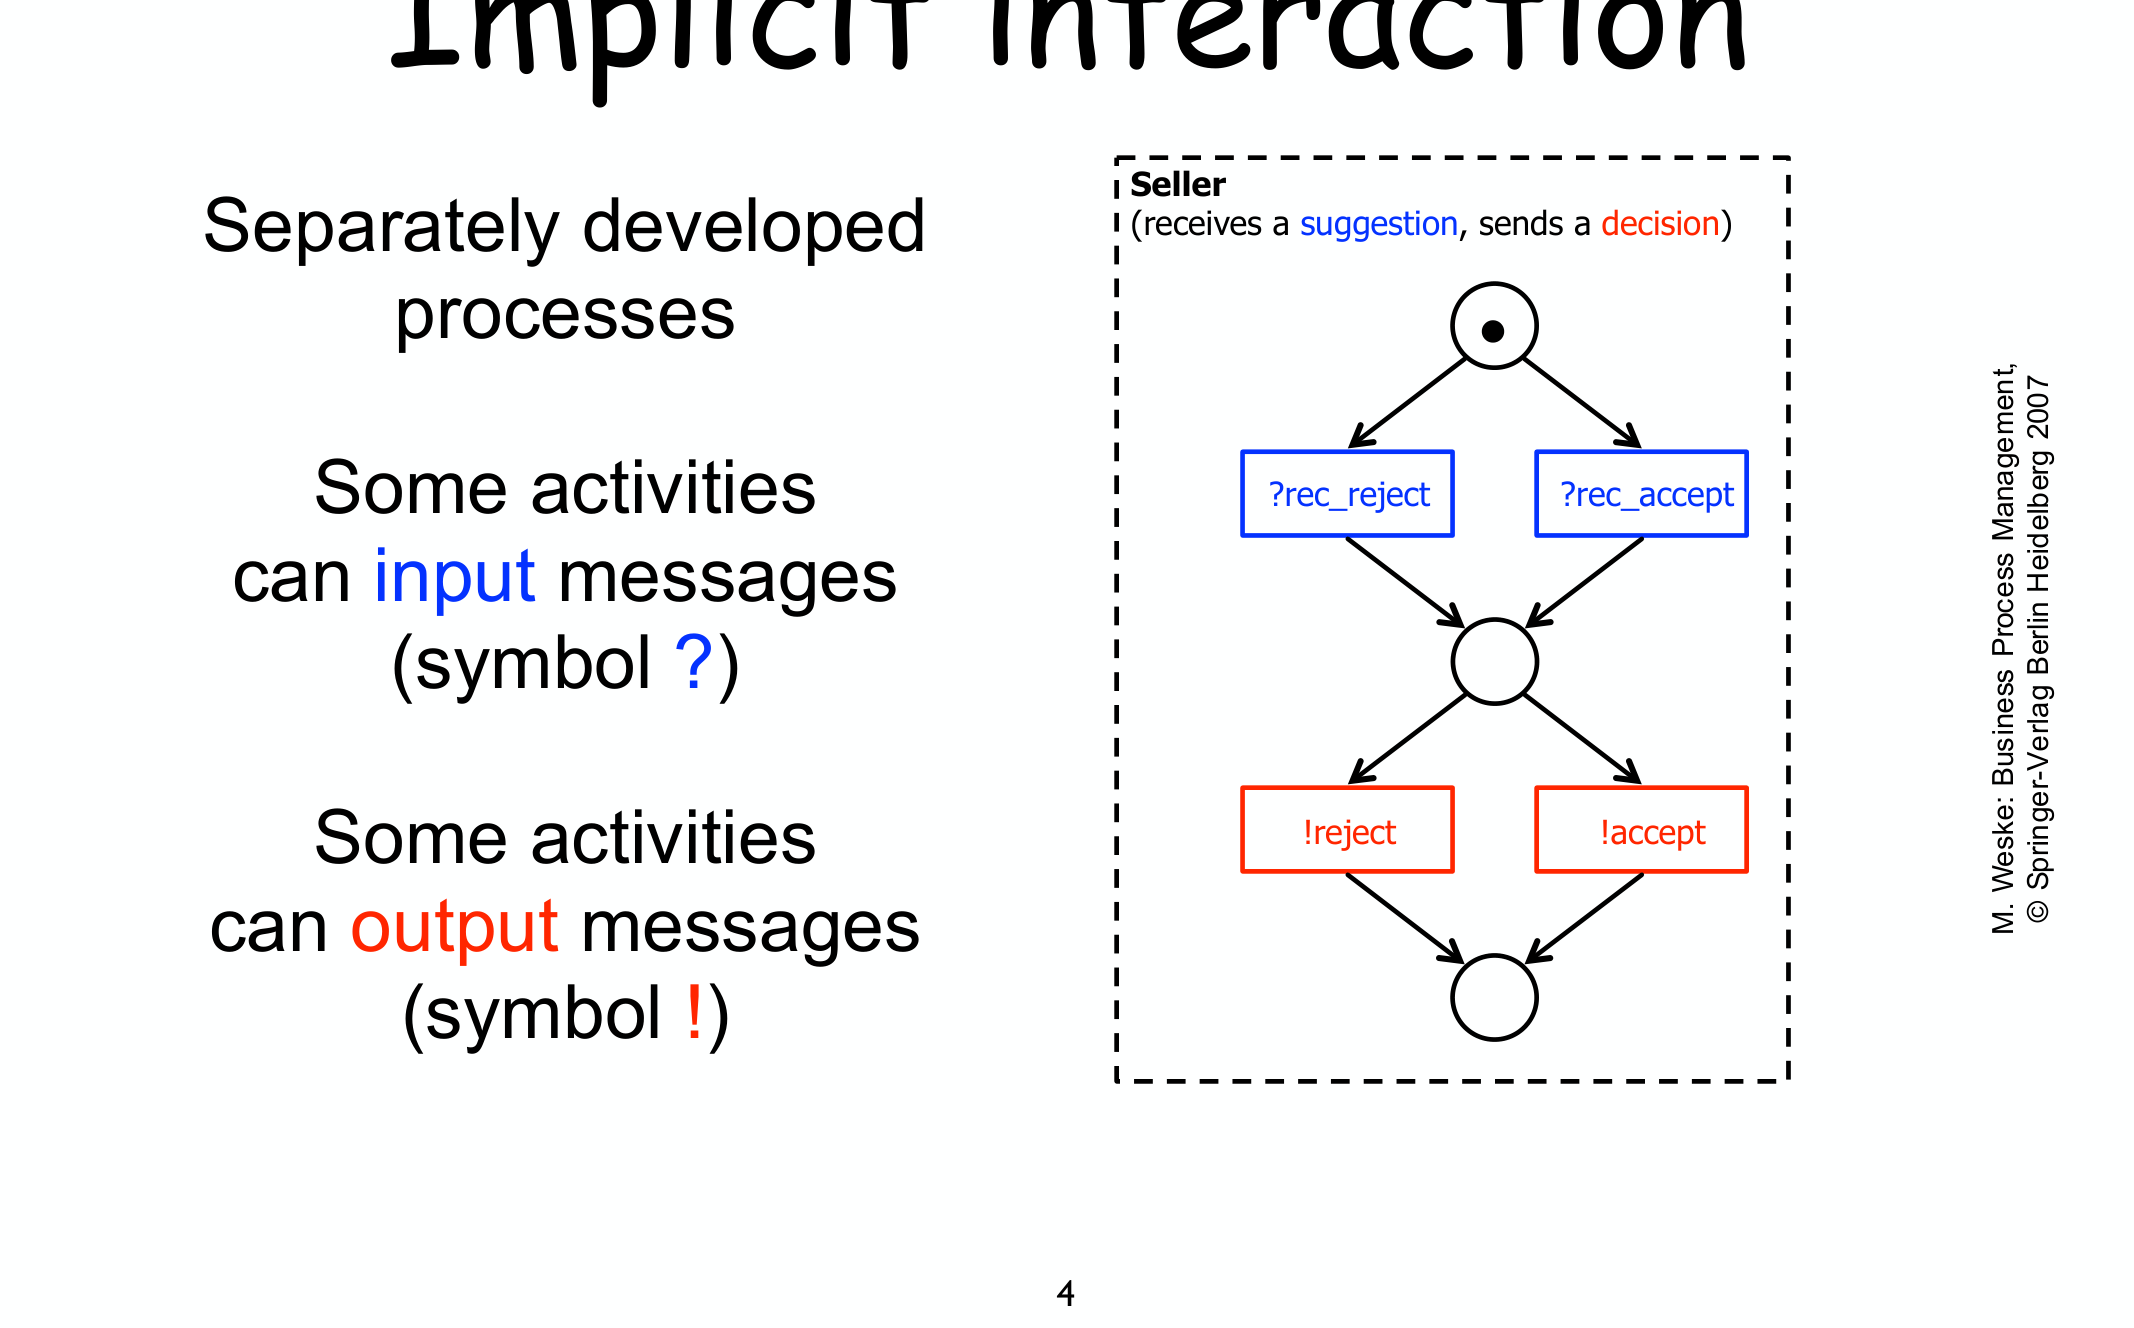
\includegraphics[width=0.74\linewidth,height=0.34\textheight,keepaspectratio]{images/18-workflow-systems_p4_implicit-interaction.png}
\caption{Il process \textbf{Seller}: riceve un suggerimento (\texttt{?rec\_accept}/\texttt{?rec\_reject}) e invia una decisione (\texttt{!accept}/\texttt{!reject}). I simboli \texttt{?}/\texttt{!} segnano dove il processo comunica con l'esterno, ma finché resta isolato non sappiamo \emph{con chi}.}
\end{figure}

\section{\texorpdfstring{Workflow module: dare forma all'interfaccia}{Workflow module: dare forma all'interfaccia}}

Per rendere l'interazione \textbf{esplicita} (e quindi analizzabile con i Petri net), i punti di ricezione e invio diventano dei \textbf{place di interfaccia}: un place di input per ogni possibile messaggio ricevuto, uno di output per ogni messaggio inviato.

\begin{boxwarning}{Attenzione: non è più un workflow net!}
Se il workflow net di partenza era \textbf{validato} (sound, magari safe), aggiungere i place di interfaccia lo trasforma in qualcosa di diverso: un workflow net ha \emph{un solo} place iniziale e \emph{uno} finale, ma ora ci sono \textbf{più punti di ingresso/uscita} (uno per ogni place di interfaccia). Serve un nuovo nome per questo oggetto: \textbf{workflow module}.
\end{boxwarning}

\begin{boxdefinition}{Workflow module}
Un workflow module consiste di: - un workflow net \textbf{sound}:

\[
(P, T, F)
\]

\begin{itemize}
\item un insieme di \textbf{place di input} $P_I$ e archi di input:
\end{itemize}

\[
F_I \subseteq (P_I \times T)
\]

\begin{itemize}
\item un insieme di \textbf{place di output} $P_O$ e archi di output:
\end{itemize}

\[
F_O \subseteq (T \times P_O)
\]

con il vincolo che \textbf{ogni transizione ha al più un arco} verso l'interfaccia ($P_I \cup P_O$) — una transizione non può scambiare più di un messaggio alla volta.
\end{boxdefinition}

\begin{figure}[!htb]
\centering
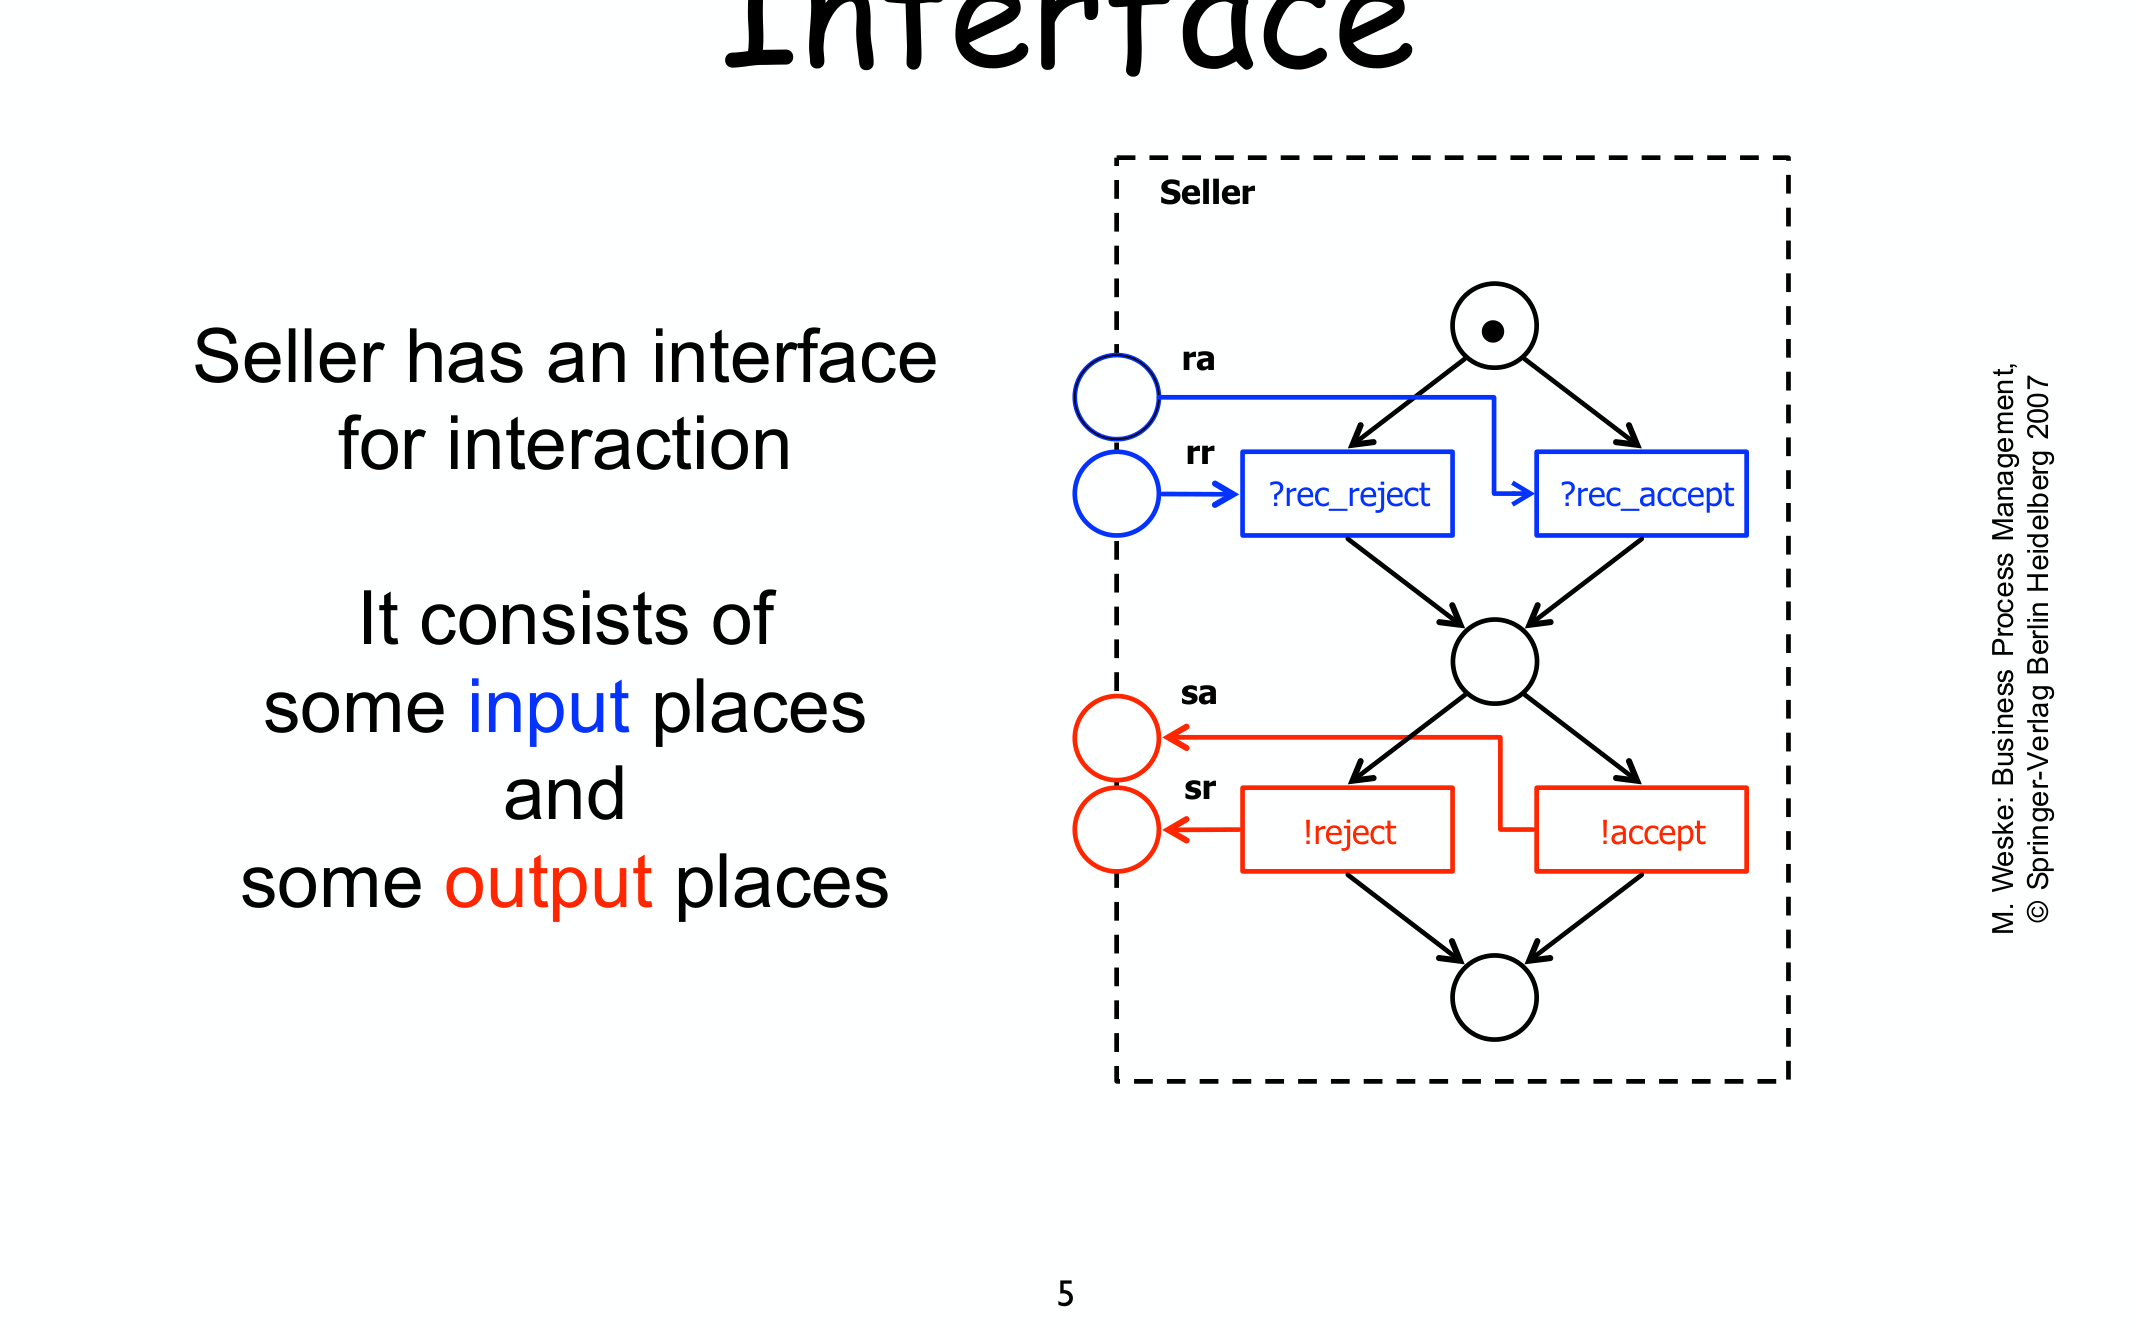
\includegraphics[width=0.74\linewidth,height=0.34\textheight,keepaspectratio]{images/18-workflow-systems_p5_interface.png}
\caption{L'\textbf{interfaccia} di Seller: i place $P_I = \{ra, rr\}$ (input, blu) alimentano le transizioni \texttt{?rec\_reject}/\texttt{?rec\_accept}; i place $P_O = \{sa, sr\}$ (output, rosso) sono riempiti da \texttt{!reject}/\texttt{!accept}. L'interfaccia è la "presa" con cui il modulo si collega ad altri.}
\end{figure}

\section{\texorpdfstring{Compatibilità strutturale e composizione}{Compatibilità strutturale e composizione}}

Un modulo da solo non fa nulla — descrive solo cosa può inviare/ricevere. Per farlo \emph{funzionare} bisogna collegarlo ad altri moduli che si scambiano gli stessi messaggi. Prima di collegarli, si controlla che le "prese" combacino.

\begin{boxdefinition}{Structural compatibility}
Un insieme di workflow module è \textbf{structurally compatible} se: - per ogni messaggio che \textbf{può essere inviato}, c'è \textbf{esattamente un} modulo che può riceverlo; - per ogni messaggio che \textbf{può essere ricevuto}, c'è \textbf{esattamente un} modulo che può inviarlo.

(si assume che i formati dei dati scambiati combacino). In pratica: ogni place di output di un modulo deve corrispondere a \textbf{uno e un solo} place di input di un altro modulo, e viceversa — nessun messaggio "orfano".
\end{boxdefinition}

Una volta verificata la compatibilità, la \textbf{composizione} è semplicissima: si \textbf{fondono} (identificano) i place di output di un modulo con i corrispondenti place di input dell'altro. Non serve nessuna transizione aggiuntiva — i place condivisi \emph{sono} il canale di comunicazione.

\begin{figure}[!htb]
\centering
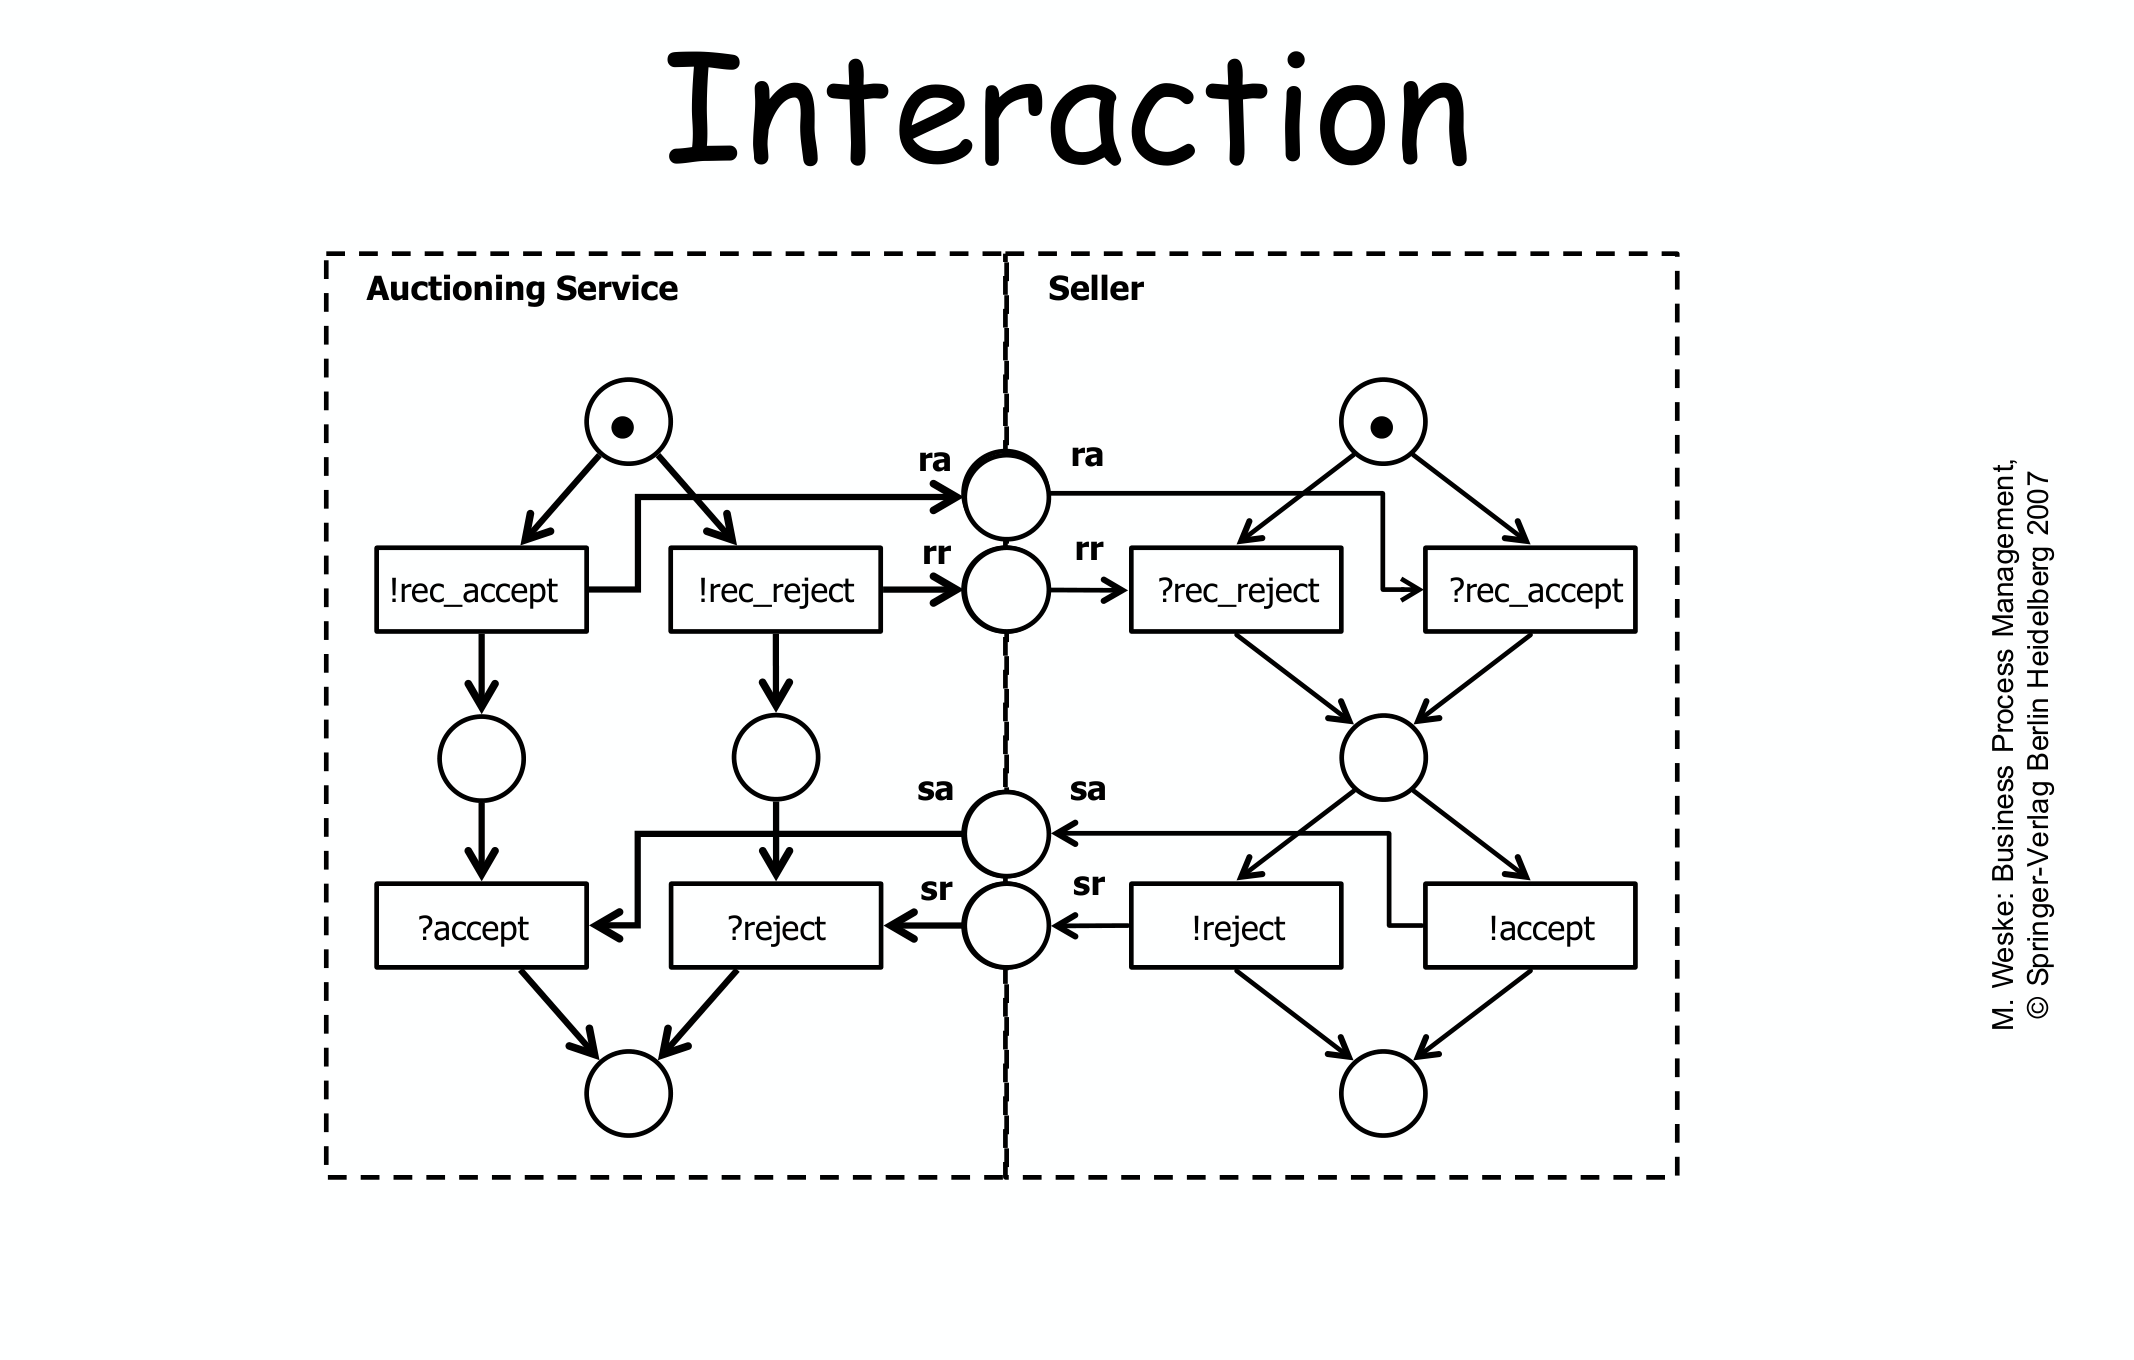
\includegraphics[width=0.74\linewidth,height=0.34\textheight,keepaspectratio]{images/18-workflow-systems_p11_interaction.png}
\caption{Compatibilità e composizione. \textbf{Auctioning Service} invia \texttt{!rec\_accept}/\texttt{!rec\_reject} sui place \texttt{ra}/\texttt{rr}, che \textbf{Seller} riceve come \texttt{?rec\_accept}/\texttt{?rec\_reject}; simmetricamente per \texttt{sa}/\texttt{sr}. Fondendo i place di interfaccia condivisi (la colonna centrale del disegno) si ottiene un'unica rete: i due moduli sono ora \textbf{collegati}.}
\end{figure}

Dopo aver fuso le interfacce resta però una domanda aperta, la stessa di \hyperref[ch:16b]{Buyer/Reseller}: \textbf{il sistema risultante si comporta bene?} E che relazione c'è con la soundness dei singoli moduli?

\section{\texorpdfstring{Workflow system: chiudere il cerchio}{Workflow system: chiudere il cerchio}}

La composizione di moduli compatibili non è ancora un workflow net "pulito": mancano ancora un unico inizio e un'unica fine globali. Si chiudono aggiungendo, come nella \hyperref[ch:12]{costruzione di $N\textasciicircum{}\star$}, un place e una transizione iniziali/finali che avvolgono l'intero sistema.

\begin{boxdefinition}{Workflow system}
Un \textbf{workflow system} è un workflow net ottenuto da $n$ workflow module \textbf{structurally compatible} (con place iniziali $i_1,\dots,i_n$ e finali $o_1,\dots,o_n$), aggiungendo: - un place iniziale $i$ e una transizione $t_i$ da $i$ a \textbf{tutti} gli $i_1,\dots,i_n$:

\[
i \ \xrightarrow{\ t_i\ }\ i_1,\dots,i_n \qquad \text{(avvia tutti i moduli in parallelo)}
\]

\begin{itemize}
\item un place finale $o$ e una transizione $t_o$ da \textbf{tutti} gli $o_1,\dots,o_n$ a $o$:
\end{itemize}

\[
o_1,\dots,o_n \ \xrightarrow{\ t_o\ }\ o \qquad \text{(attende che tutti i moduli terminino)}
\]

La marcatura iniziale è un token in $i$.
\end{boxdefinition}

\begin{figure}[!htb]
\centering
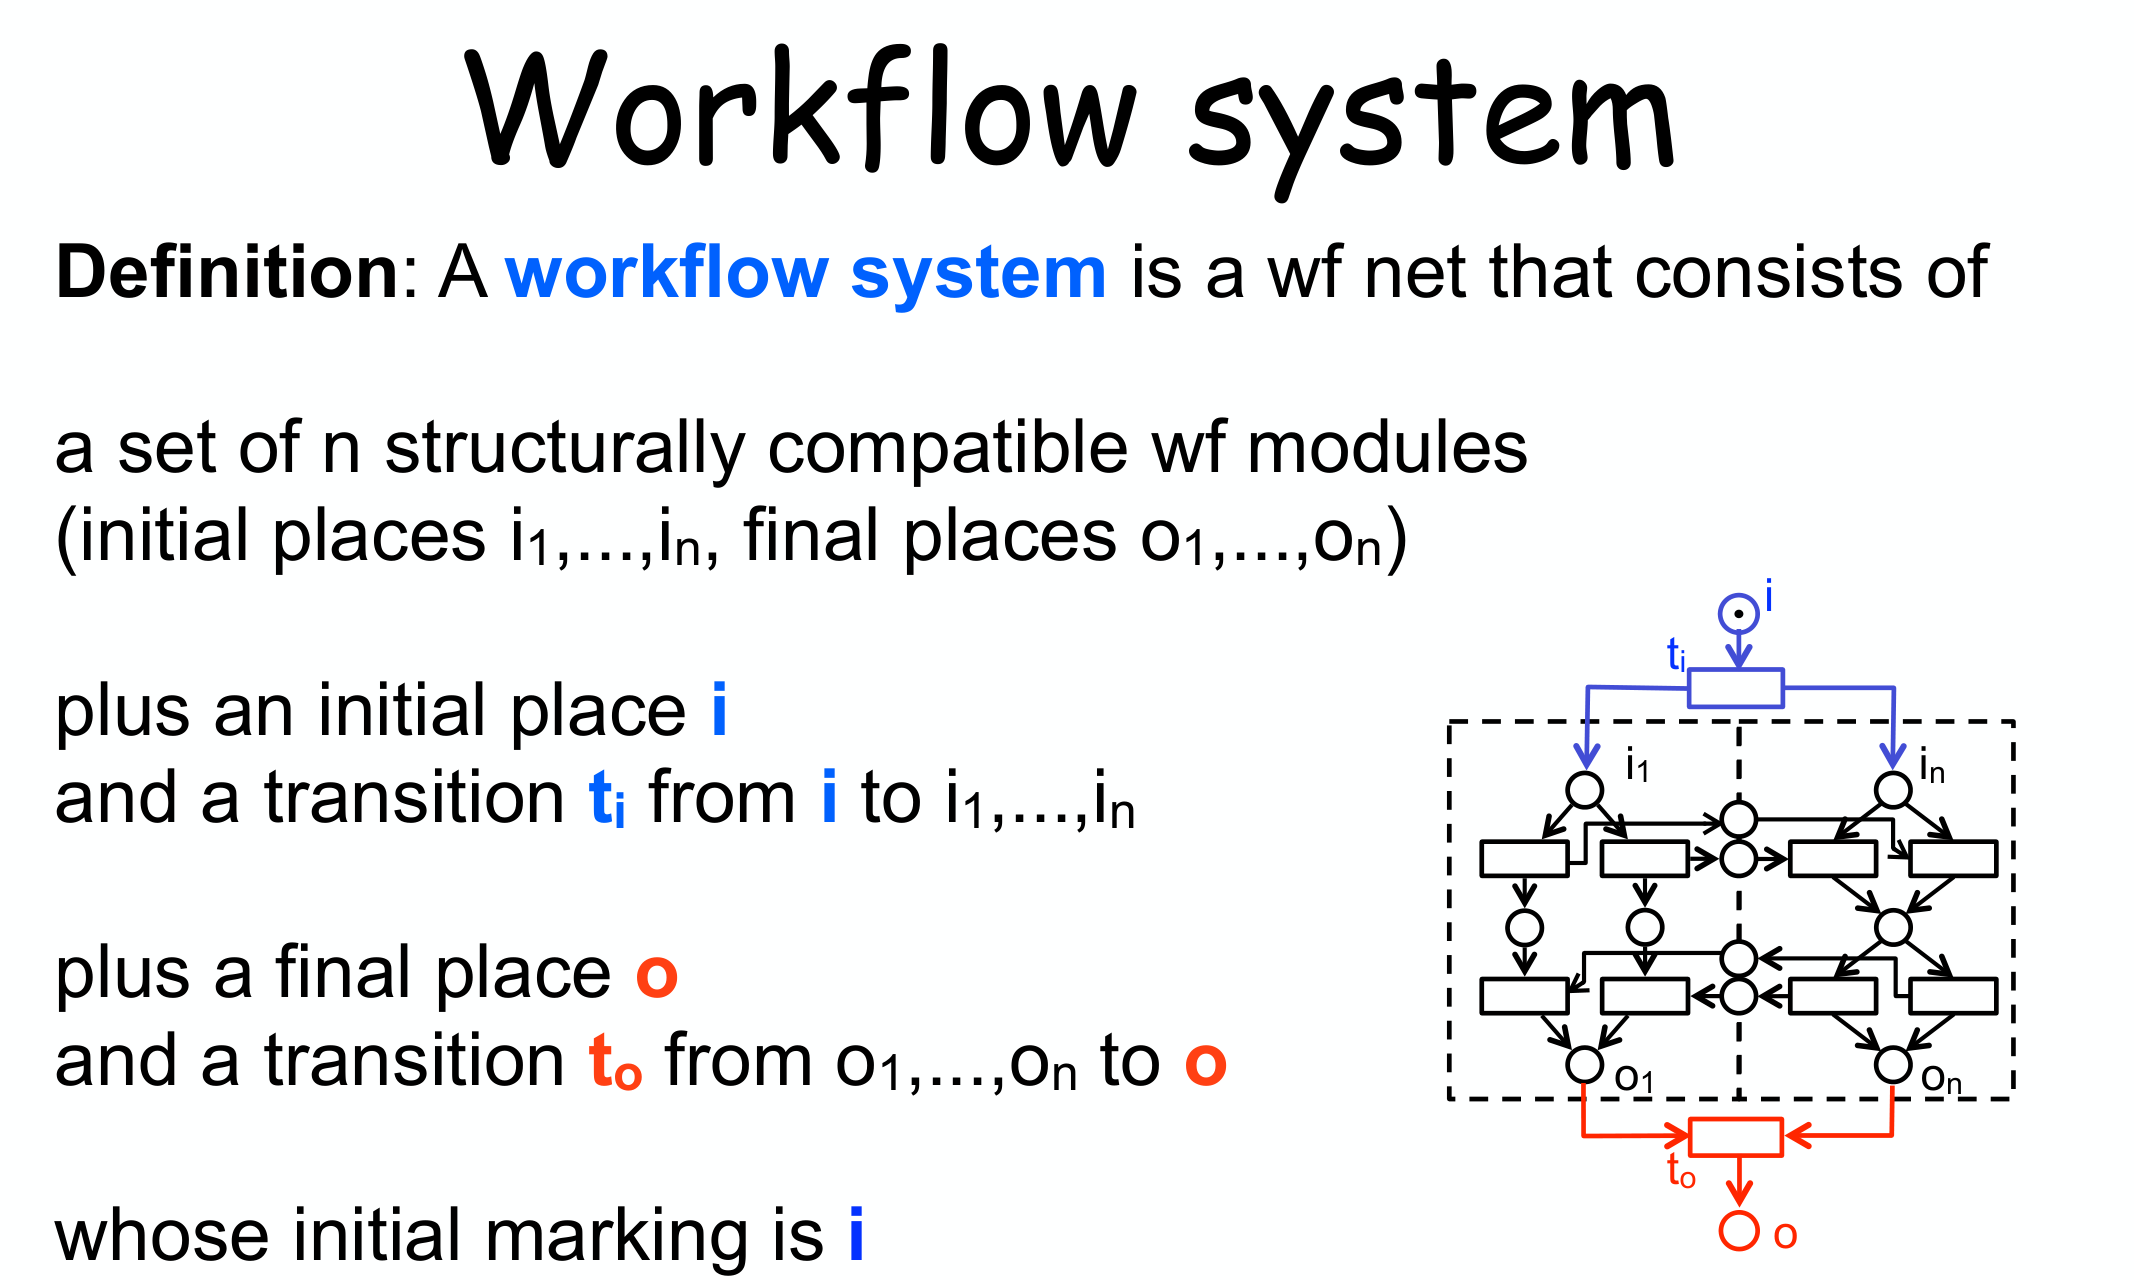
\includegraphics[width=0.74\linewidth,height=0.34\textheight,keepaspectratio]{images/18-workflow-systems_p15_workflow-system-def.png}
\caption{Struttura di un workflow system: $t_i$ "lancia" simultaneamente tutti i moduli, $t_o$ aspetta che \textbf{tutti} abbiano finito. È esattamente l'analogo multi-modulo del singolo workflow net $i \to o$.}
\end{figure}

Il punto cruciale — e la ragione per cui tutta questa macchina serve — è che \textbf{un workflow system è, a tutti gli effetti, un ordinario workflow net}. Quindi la sua soundness si verifica \textbf{esattamente come sempre}: liveness e boundedness di $(N^\star)$, nessuno strumento nuovo.

\begin{boxexample}{Sound + Sound può dare non sound}
Componendo \textbf{Auctioning Service} e \textbf{Seller} (entrambi sound singolarmente) si ottiene un workflow system che, controllato, risulta \textbf{non sound} — la comunicazione introduce un deadlock che non esisteva nei singoli moduli. Modificando leggermente uno dei due moduli (\textbf{Auctioning Service'}), il sistema composto torna \textbf{sound}. La morale, già anticipata in \hyperref[ch:16b]{16b — BPMN Analysis}, si dimostra ora con lo strumento giusto: \textbf{la soundness dei singoli moduli non implica quella del sistema}; va sempre controllata sul workflow system risultante dalla composizione.
\end{boxexample}

\section{\texorpdfstring{Il problema della soundness "piena": weak soundness}{Il problema della soundness "piena": weak soundness}}

C'è però un disagio pratico nell'esigere la soundness piena sul sistema composto. I workflow module sono pensati per essere \textbf{sviluppati separatamente} e \textbf{riusati} in sistemi diversi: è normale che, in un dato system, \textbf{non tutte} le funzionalità offerte da un modulo vengano usate. Un task del modulo che in \emph{questo} particolare sistema non serve mai risulterebbe \textbf{dead} — e la soundness piena lo vieterebbe categoricamente (condizione "no dead task").

\begin{boxwarning}{Perché la soundness piena è troppo esigente qui}
Pretendere \textbf{zero task dead} nel sistema composto è irrealistico quando i moduli sono generici e riusabili: alcune loro funzionalità restano naturalmente inutilizzate in un contesto specifico, senza che questo comprometta la correttezza dell'interazione.
\end{boxwarning}

Si introduce quindi una nozione più permissiva, che rilassa \textbf{solo} la condizione sui dead task:

\begin{boxdefinition}{Weak soundness}
Un workflow net è \textbf{weak sound} se soddisfa \textbf{option to complete} e \textbf{proper completion} (\hyperref[ch:12]{le condizioni 2 e 3} della soundness) — ma \textbf{ammette task dead} (rilassa la condizione 1).

Si verifica sul reachability graph esattamente come la soundness piena. Garantisce comunque \textbf{deadlock-freedom} e la \textbf{corretta terminazione} di tutti i moduli — solo non garantisce che ogni singolo task venga mai eseguito.
\end{boxdefinition}

\begin{boxtip}{Sound + Sound = weak sound (nell'esempio)}
Nell'esempio del sistema \emph{non sound} visto sopra: il difetto non era un deadlock o una terminazione sporca, ma la presenza di \textbf{task dead} nel sistema composto (funzionalità di un modulo non attivate in questo particolare abbinamento). Il sistema \textbf{non è sound}, ma \textbf{è weak sound}: nessun blocco, nessun token pendente — solo qualche task inutilizzato, che è accettabile per moduli pensati per essere generici.
\end{boxtip}

\section{\texorpdfstring{Riepilogo}{Riepilogo}}

\begin{boxabstract}{Il quadro}
\begin{itemize}
\item Un \textbf{workflow module} = workflow net sound + interfaccia (place di input/output per i messaggi).
\item Più moduli \textbf{structurally compatible} si compongono fondendo i place di interfaccia condivisi.
\item Chiudendo con $i,t_i$ e $o,t_o$ si ottiene un \textbf{workflow system} — un workflow net a tutti gli effetti, verificabile con gli strumenti soliti.
\item \textbf{Sound + sound non implica sound}: la composizione va sempre controllata sul sistema intero.
\item La \textbf{weak soundness} (option to complete + proper completion, senza "no dead task") è il criterio realistico per sistemi fatti di moduli riusabili.
\end{itemize}
\end{boxabstract}

Con moduli e sistemi possiamo modellare processi che comunicano; resta però aperta la questione opposta: dato un log di eventi reali, \textbf{quanto bene} il modello descrive ciò che accade davvero? Se ne occupa la prossima lezione. $\rightarrow$ \hyperref[ch:19]{19 — Conformance}